\documentclass[letterpaper,12pt]{article}
\usepackage{lipsum}  
\usepackage{graphicx}
\usepackage{subcaption}
\usepackage[english]{babel}
\usepackage{fancyhdr}

\graphicspath {{figures/}}

\setlength{\headheight}{15pt}

\pagestyle{fancy}
\fancyhf{}
\lhead{\textbf{Version:} 1  \textbf{Revision:} \today}
\rhead{\thepage}
\lfoot{Cole Kampa}
\rfoot{\textit{Mu2e: University of Minnesota}}

\renewcommand{\footrulewidth}{1pt}


\begin{document}
\begin{titlepage}
	\centering
	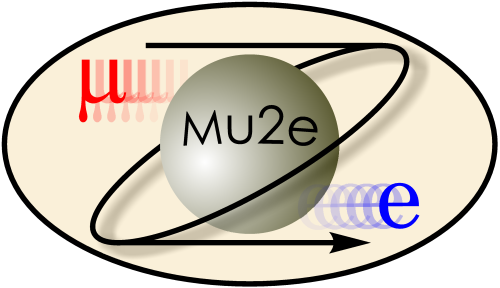
\includegraphics[width=0.5\textwidth]{mu2e_logo_oval.png}\par\vspace{2cm}
	{\scshape\LARGE Automated Sense Wire Tensioner: \\ Project Status Update 1\par}
	\vspace{3cm}
	{\Large Cole Kampa\par}
	%\vspace{3cm}
	\vspace{3.5cm}
	{\large University of Minnesota\par}
 	\vspace{.5cm}
	{\large \today \par}
	% Bottom of the page
	\vfill
	{kampa041@umn.edu\par}
\end{titlepage}

\clearpage
\setcounter{page}{2}


\section*{Status \& Milestones}
See Images section for labeled test setup pictures.
\begin{itemize}
\item{\textbf{Resolution \& Time:} $(80.0\pm 0.5)$gf in 5-10 seconds (running circuit)
}
%\item{\textbf{Current setup:} Actuator and load cell on opposite sides, used as two attachment points for sense wire/thread. Thread is already attached with hot glue on the actuator end (wire pulling). Circuit built on solderless breadboard. Simple controls: serial signal or push button to start and stop tensioning. Piezzo buzzer and LEDs for warnings/alerts to user.
%}
\item{\textbf{Cost Estimate:} Electronics: $\mathcal{O}(\$100)$; Manufacturing (tracks and platform): unknown, dependent on desired position precision
}
\item{\textbf{Next Steps:} finish actuator platform; design attachment for load cell to actuator; try current setup with test panel
}
\end{itemize}

\section*{Advantages \small{(vs. Hanging Masses)}}
\begin{itemize}
\item{No pulleys (after sense wire is through a straw)
}
\item{Easier operation: track system vs. moving pulleys between holes; being able to see the sense wire becomes unnecessary except at the point of clamping the wire with stiff spring (not in current setup)
}
\item{May save non-trivial amounts of sense wire
}
\item{Scalability to speed process up even more; i.e. with 6 tension devices on a panel track, each row needs to run tensioner 8 times rather than 48
}
\end{itemize}

\section*{Current Problems}
\begin{itemize}
\item{
Load cell is currently on opposite end of straw and acts as one of the fixed points. If the load cell can be attached directly to the actuator, we could clamp the wire with a spring on one end (like the current method). This saves the step of having to hot glue another thread to the sense wire to attach to the load cell.
}
\item{
Mounts not completed and slow to progress. I am unable to work in the student shop (currently enrolled in 6 week course to get access), so others have been helping when they get time.
}
\item{
Since a test with a panel has not been setup, other logistical issues will likely arise with more testing.
}
\end{itemize}

\section*{Images}
\begin{figure} [h]
		\centering
		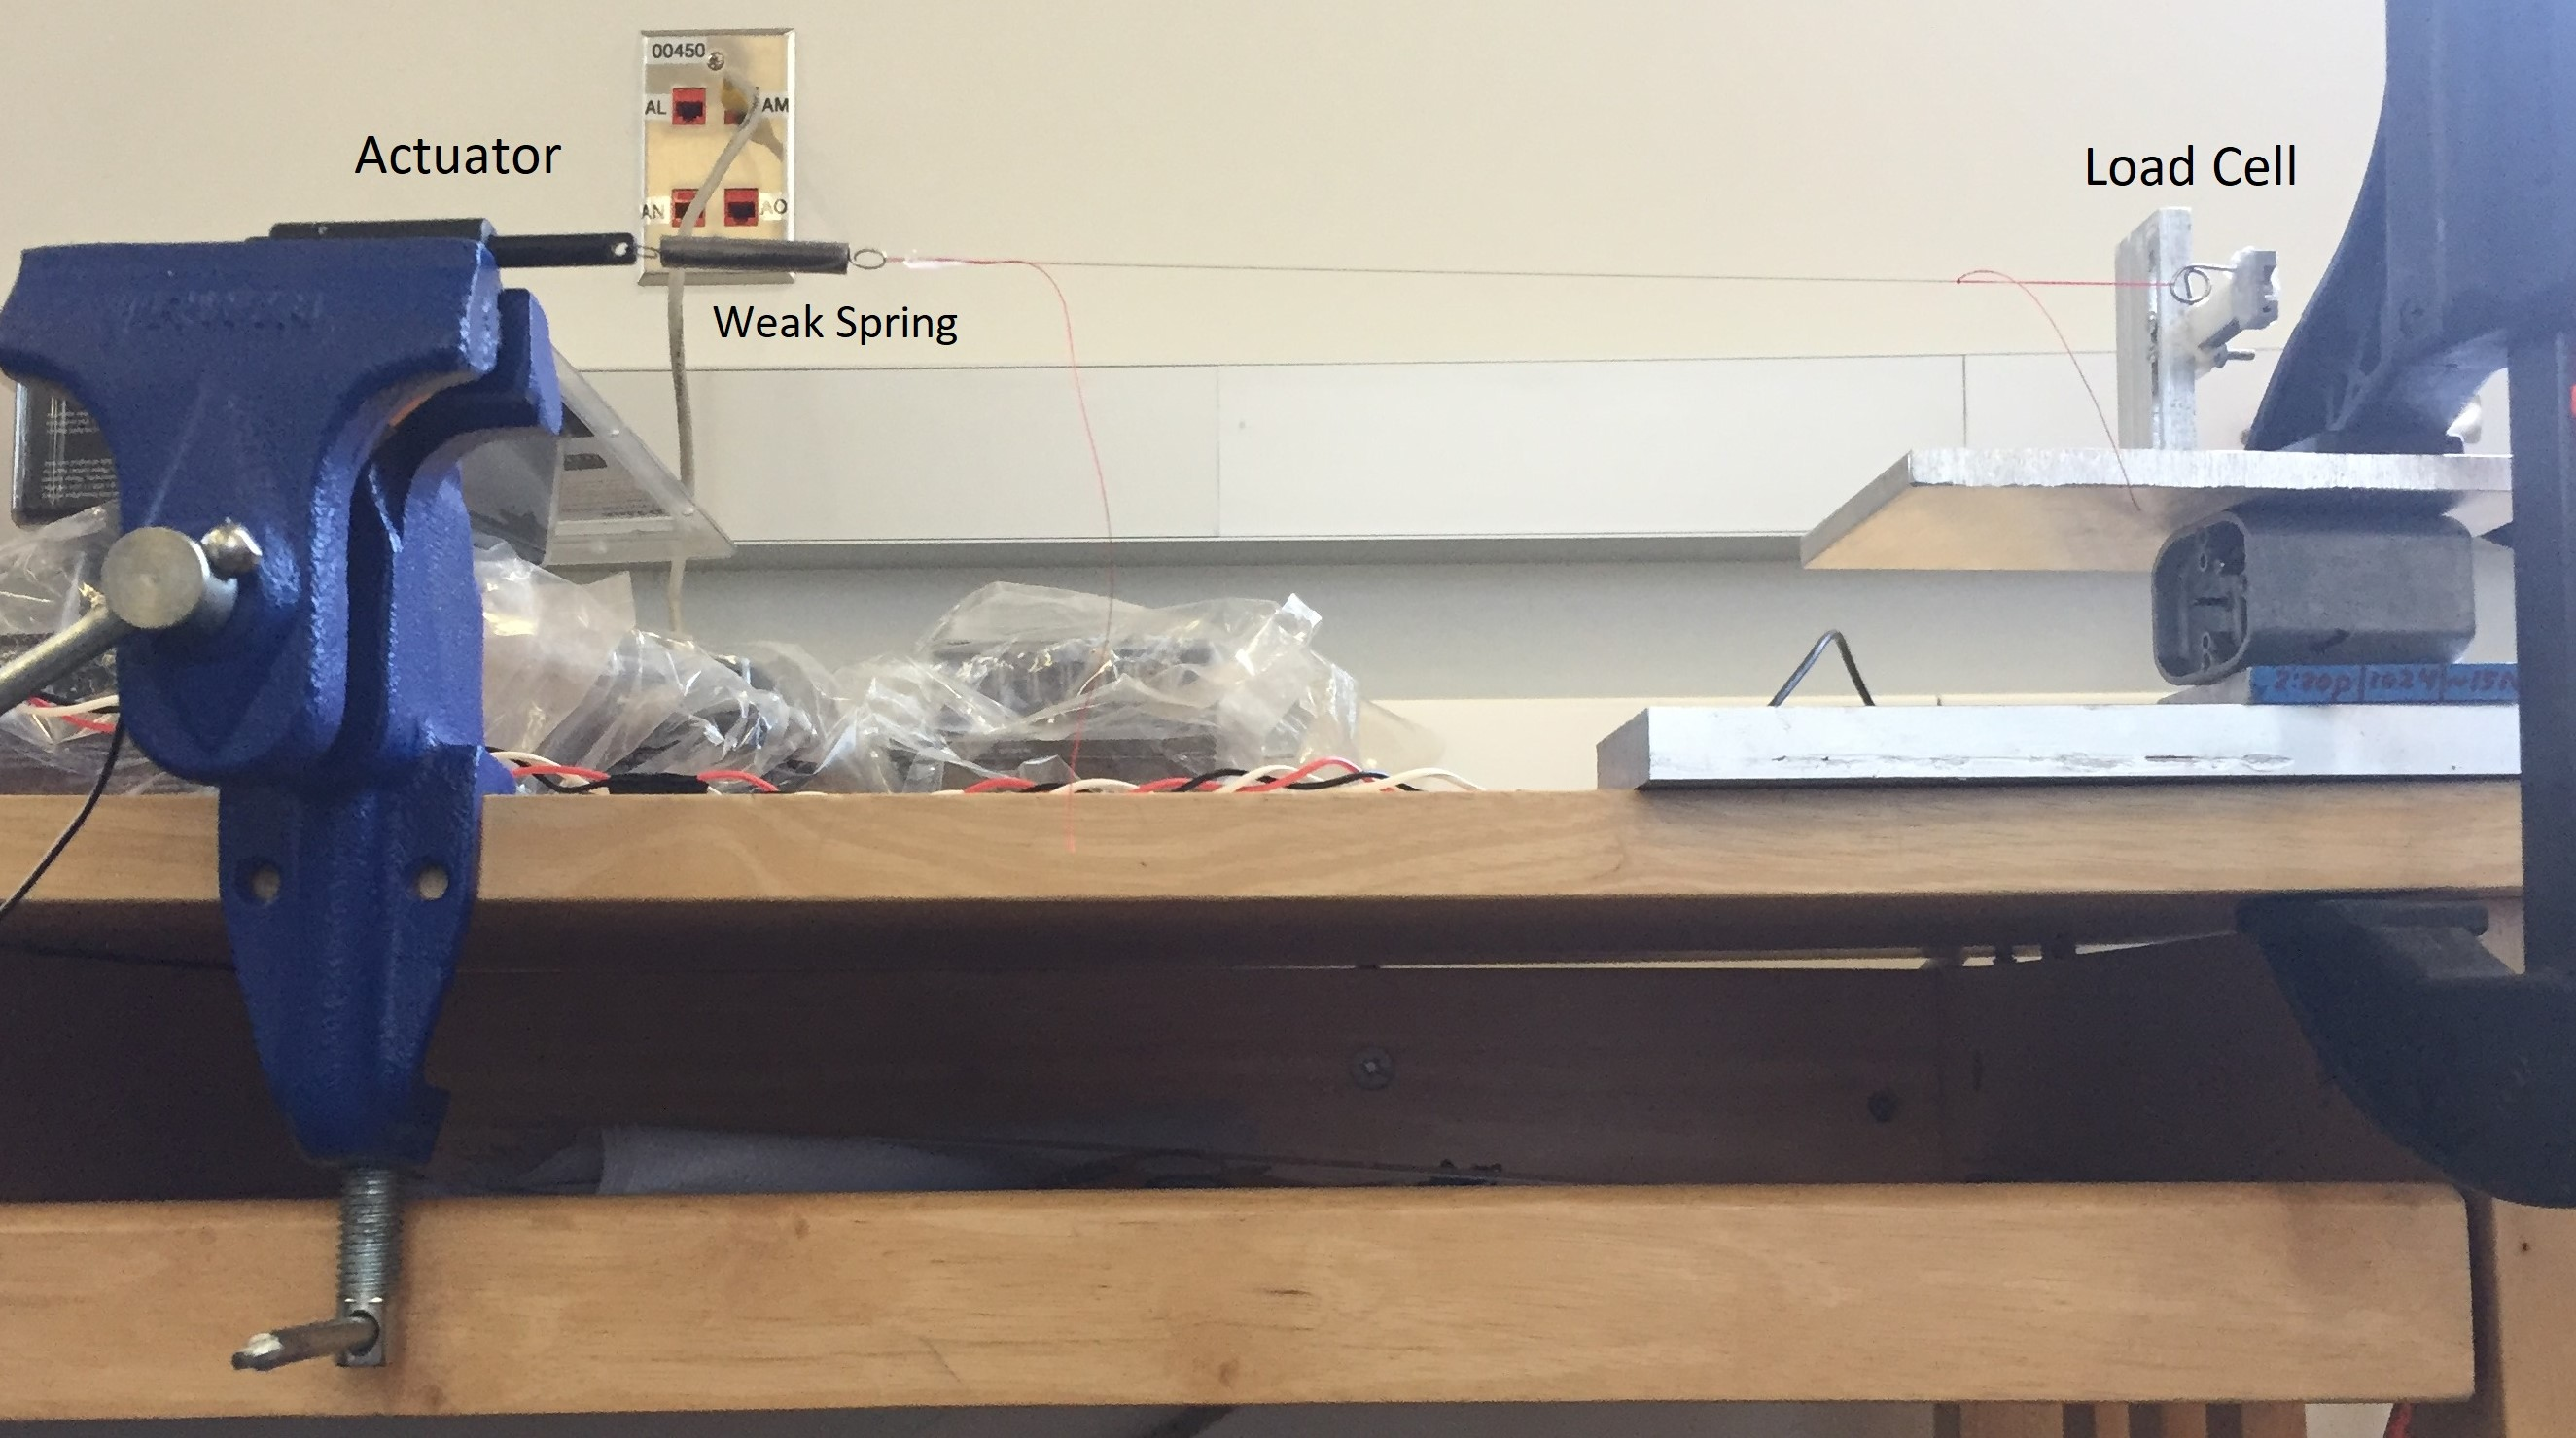
\includegraphics[width=\textwidth]{setup_side.jpg}
		\caption{Test setup using thread only. Verified tests work on old sense wire (brittle).}
		\label{fig:side}
\end{figure}
\begin{figure}[!h]
	\centering
	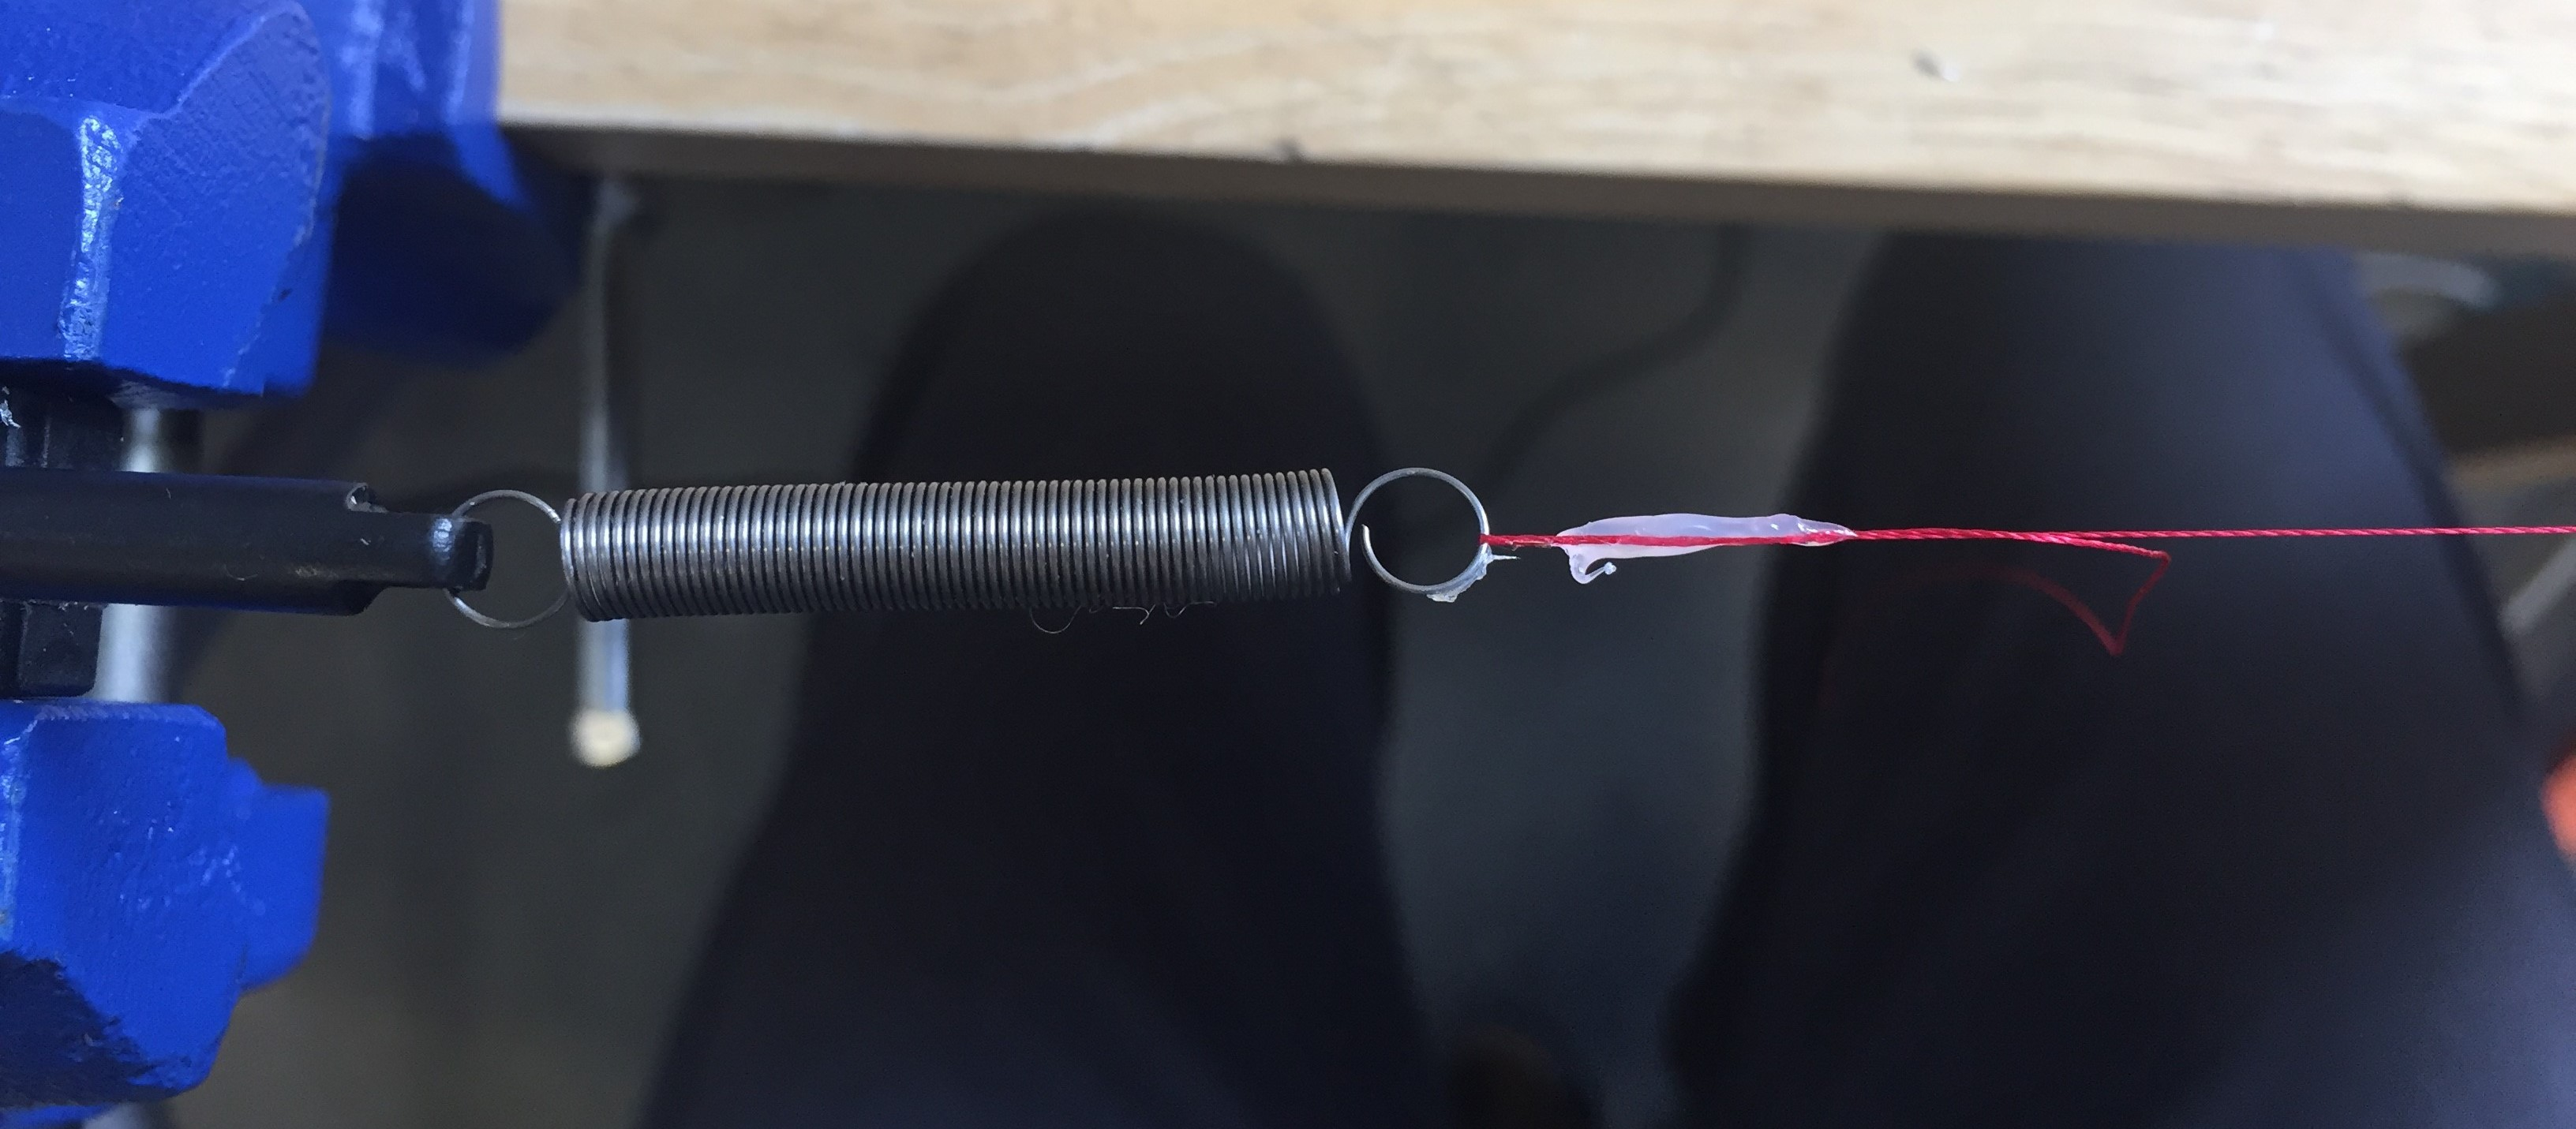
\includegraphics[width=0.75\textwidth]{thread_glue.jpg}
	\caption{After passing thread (glued to sense wire) through spring, a small amount of hot glue holds the looped thread in place for tensioning.}
	\label{fig:glue}
\end{figure}
\begin{figure}[h]
	\centering
	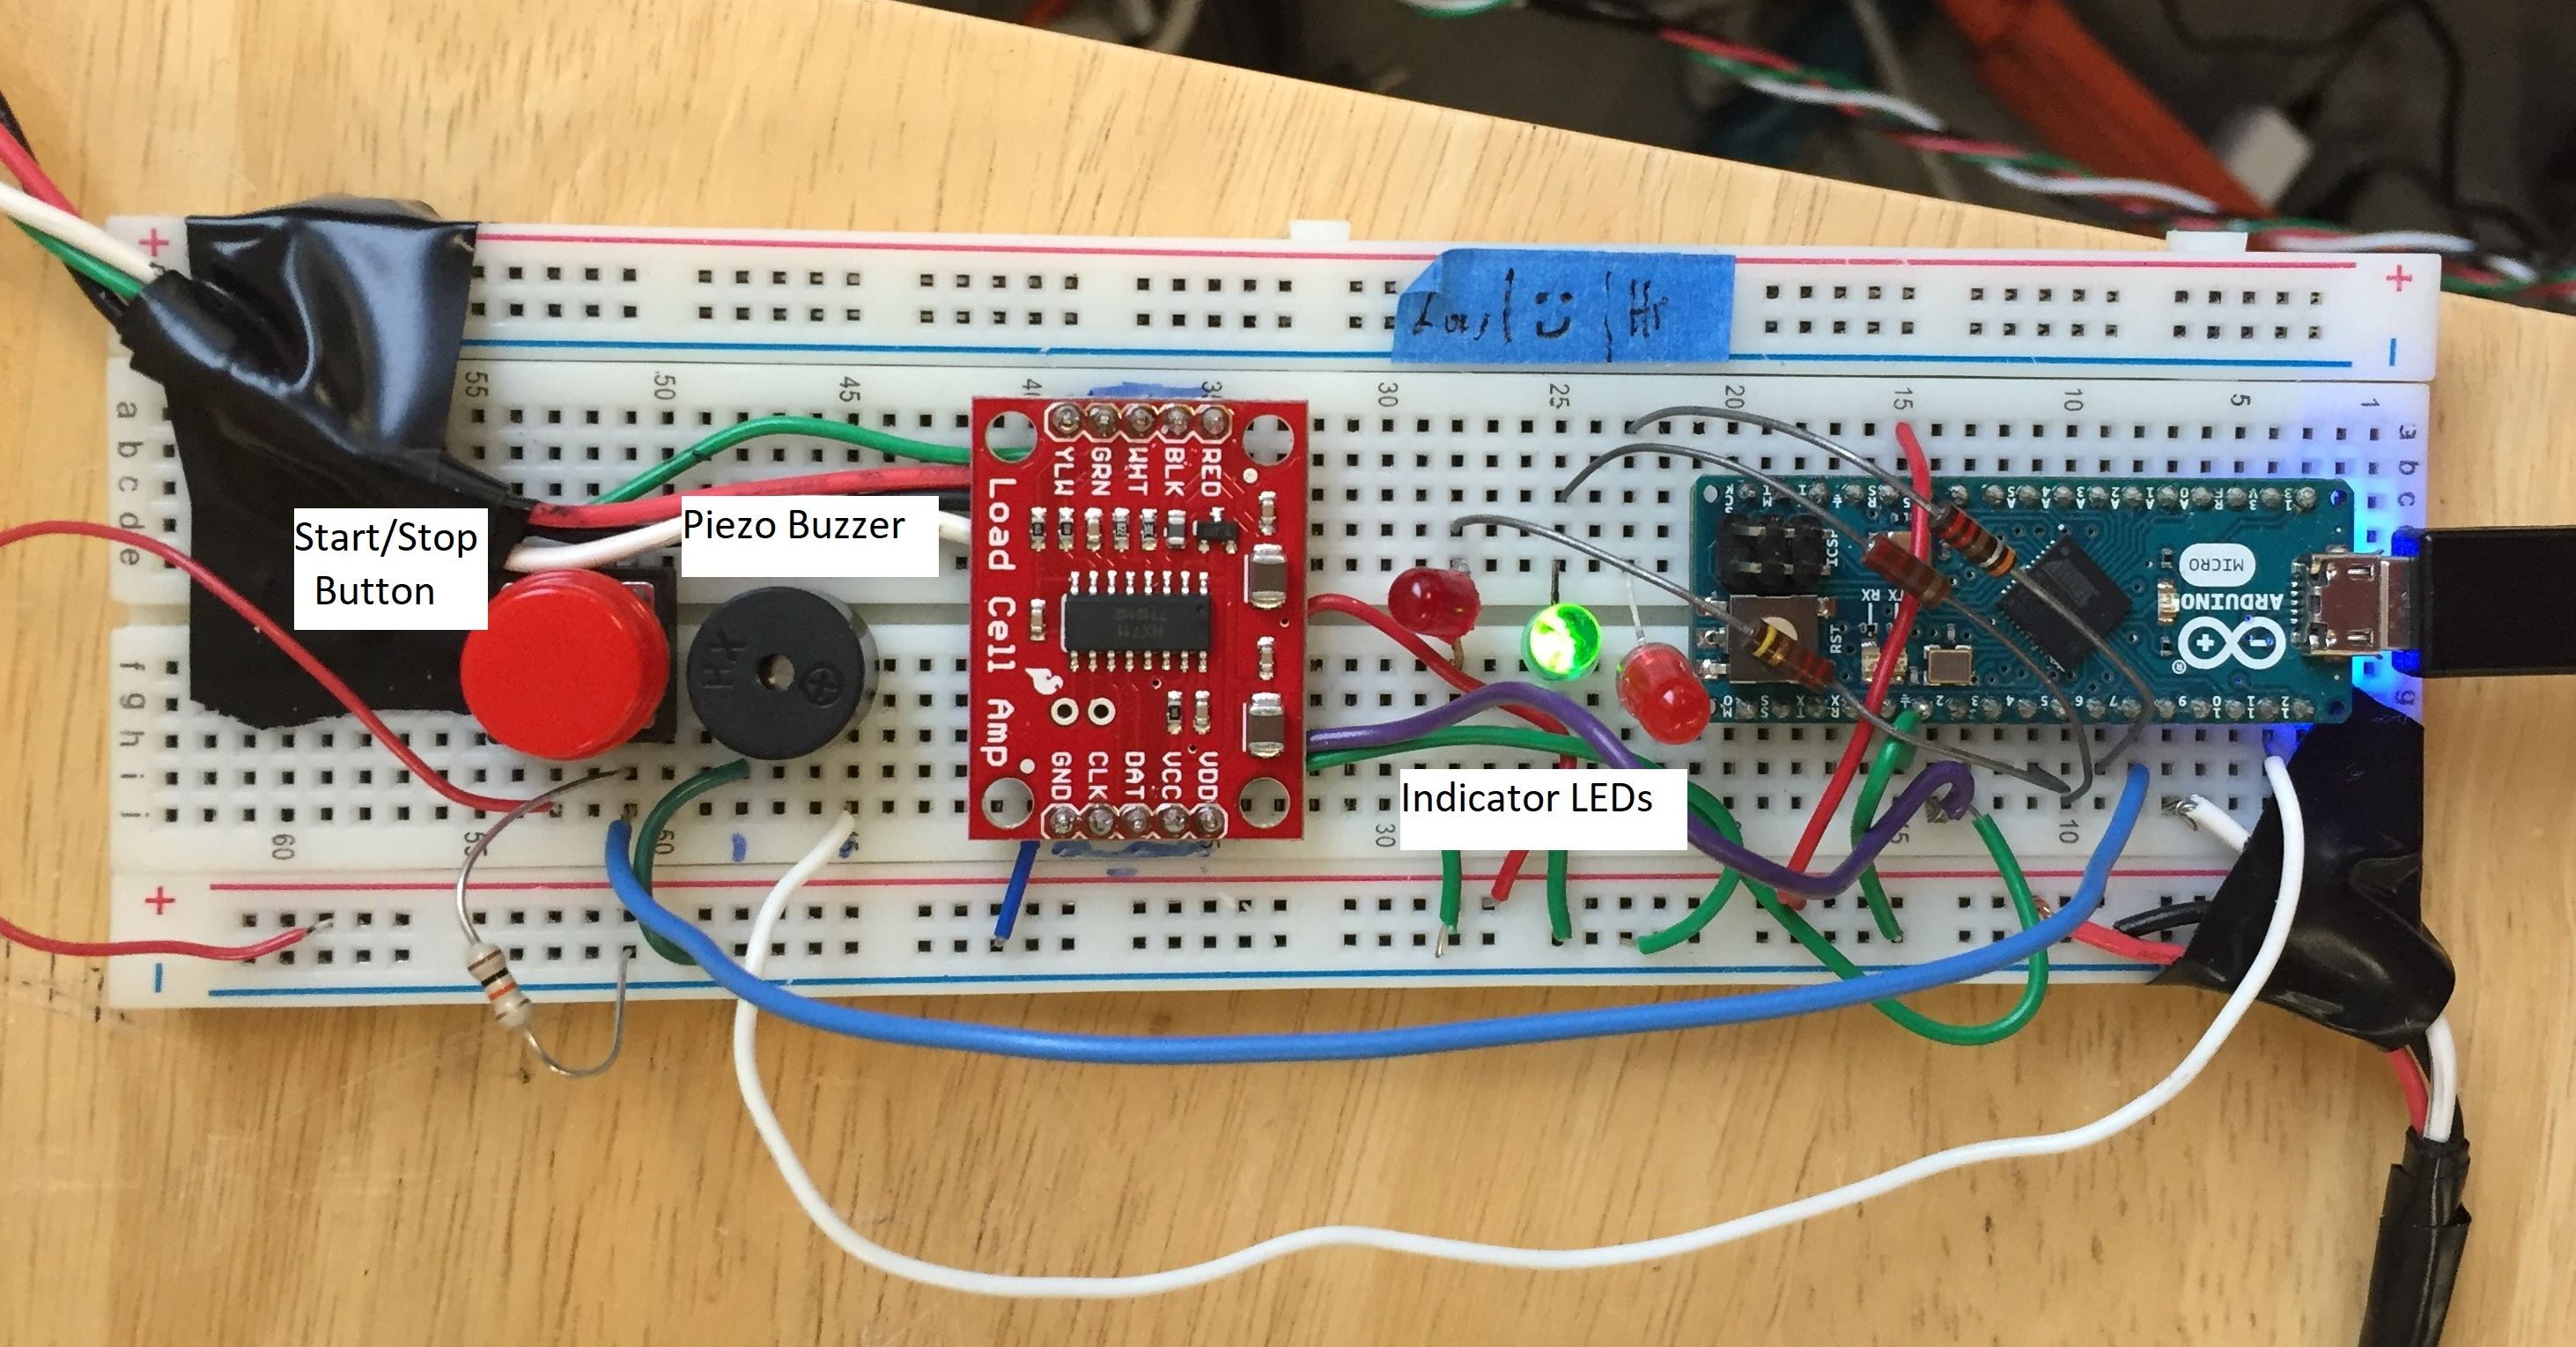
\includegraphics[width=\textwidth]{circuit_top.jpg}
	\caption{Prototype circuit. All analog pins and 3-4 digital pins are available for further additions.}
	\label{fig:circuit}
\end{figure}



\end{document}